% !TeX spellcheck = ru_RU
% !TEX root = vkr.tex

В рамках учебной практики третьего курса автором был предложен новый алгоритм для решения задачи достижимости, основанный на классическом алгоритме поиска в ширину для нескольких стартовых вершин~\cite{method_msbfs}.

Идея алгоритма состоит в последовательном применении операции умножения матриц для совершения шага в алгоритме поиска в ширину. На примере~\ref{ex_graphblas} показано, как шаг в алгоритме поиска в ширину выражается с помощью операции умножения матрицы на вектор.

\begin{figure}[h!]
  \centering
  \includegraphics[width=0.7\linewidth]{pictures/AdjacencyMatrixGraphBLASBFS.png}
  \caption{Пример вычисления шага в алгоритме поиска в ширину, источник~\cite{method_gb_wiki}.}
\end{figure}\label{ex_graphblas}

Представленный далее алгоритм расширяет эту идею и применяет её для одновременного обхода графа и автомата, выражающего ограничения, заданные с помощью регулярного языка.

\subsection{Описание алгоритма}

Пусть дан граф $\mathcal{G} = \langle V, E, L\rangle$, регулярный язык, описывающий ограничения на пути в нем, и множество начальных вершин $V_{s}$ графа.
Известно, что регулярный язык может быть представлен с помощью детерминированного конечного автомата. Также известно, что конечный автомат может быть представлен с помощью графа с дополнительной информацией о стартовых и финальных состояниях. Представим полученный граф в виде матрицы смежности. Тогда регулярные ограничения могут быть выражены с помощью матрицы, ячейки которой описывают наличие перехода между двумя состояниями.  Более того, для задачи достижимости достаточно хранить в матрице смежности на $(i, j)$ месте два значения: $0$ --- отсутствие пути между вершинами $i$ и $j$, $1$ --- наличие пути.

Пусть каждой метке $l$ графа будет сопоставлена булева матрица смежности. Далее, будем оперировать с булевой декомпозицией матриц смежности $\mathcal{M}_A$ конечного автомата, и булевой декомпозицией матриц смежности $\mathcal{M}_G$ входного графа.

Алгоритм строит прямую сумму для матриц смежности $\mathcal{G}$ и $\mathcal{R}$. Представление в виде прямой суммы позволяет одновременно совершать шаг в алгоритме поиска в ширину на графе $\mathcal{G}$ и проверять удовлетворение регулярным ограничениям. Для каждого символа из пересечения множеств меток графа и алфавита регулярного языка построим матрицу $\mathcal{D} = \mathcal{M}_A \bigoplus \mathcal{M}_G$.

\begin{equation}
  \mathcal{D} =
  \left[
    \begin{matrix}
      \mathcal{M}_A & 0             \\
      0             & \mathcal{M}_G
    \end{matrix}
    \right]
\end{equation}

Далее, опишем процедуру обхода, основанную на серии умножений матрицы смежности.
В классической версии обхода используется вектор $v$, куда записывается фронт обхода графа. Так, один раз перемножая матрицу смежности на вектор $v$, можно совершать один шаг в обходе графа, как было показано в примере~\ref{ex_graphblas}.

Пусть $k$ --- количество вершин в графе, построенном по конечному автомату, $n$ --- количество вершин в графе $\mathcal{G}$. Тогда первые $k$ элементов вектора $v$ хранят информацию о номере состояния конечного автомата, построенного по $\mathcal{R}$, оставшиеся $n$ элементов хранят информацию о номере вершины входного графа. При этом для проверки путей на соответствие входным регулярным ограничениям необходимо иметь информацию о парах $(v_i, v_j)$, $0<= i < k, k <= j < k+n$. Каждая из этих пар хранит информацию о том, в каком состоянии $v_i$ мы оказались, достигнув вершину $v_j$. Предлагается разложить вектор $v$ во множество векторов $v^{0}, v^{1}, ... v^{k}$ и получить матрицу $M$ вида.

\begin{equation}
  M^{k \times (k + n)} =
  \left[
    \begin{matrix}
      v^{0} \\
      v^{1} \\
      \dots \\
      v^{k}
    \end{matrix}
    \right]
\end{equation}

Построенная таким образом матрица $M$ содержит информацию о достигнутых во время обхода вершинах графа. Остается лишь ограничить левую часть векторов $v^i$ таким образом, чтобы они всегда содержали только одну единицу, что позволит определить в каком состоянии вершина была достигнута. Для этого скажем, что $v^i[i] = 1$, $v^i[j] = 0$ при $i \neq j$. Тогда $v^i$ будет соответствовать $i$ номеру состояния $\mathcal{R}$, и правая часть вектора $v^i$ будет содержать информацию о достижимых вершинах. Матрица $M$ примет вид.

\begin{equation}
  M^{k \times (k + n)} =
  \left[
    \begin{matrix}
      Id_k & Matrix_{k \times n }
    \end{matrix}
    \right]
\end{equation}

Где $Id_k$ --- единичная матрица, $Matrix_{k \times n }$ --- матрица, хранящая фронт вершин в графе для каждого состояния.

В итоге остается проинициализировать множество начальных вершин. Для этого нужно, чтобы в ячейке $(i, i+j+1)$ матрицы $M$ стояла 1, если состояние конечного автомата, построенного по $\mathcal{R}$, соответствующее номеру $i$, является начальным, а вершина графа $\mathcal{G}$ соответствующая номеру $j$ содержится в множестве начальных вершин, то есть $j \in V_{s}$.

Перейдем к построению алгоритма, который представлен на листинге~\ref{BFSRPQ1}. На вход алгоритм принимает граф и ограничения в виде регулярного языка, которые можно представить с помощью конечного автомата.

Алгоритм обхода заключается в последовательном умножении матрицы $M$ текущего фронта на матрицу $\mathcal{D}$. В результате чего, получается матрица $M'$ содержащая информацию о вершинах, достижимых на следующем шаге. Далее, с помощью операций перестановки и сложения векторов $M'$ преобразуется к виду матрицы $M$ и присваивается ей для совершения нового шага.
Важно отметить, что на каждом шаге хранится матрица $M_{all}$, которая наполняется значениями, полученными на текущем шаге. Итерации продолжаются пока меняется $M_{all}$.

\begin{algorithm}[t]
  \caption{Алгоритм в терминах линейной алгебры
    для поиска путей от нескольких стартовых
    вершин с регулярными ограничениями}\label{BFSRPQ1}
  \begin{algorithmic}[1]
    \Procedure{MSBFS~} {$\mathcal{R}=\langle Q, \Sigma, P, F, Q_{s} \rangle,\mathcal{G}=\langle V, E, L \rangle, V_{s}$}

    \State $k\gets |Q|$, $n\gets |V|$
    \State $\mathcal{M}_A\gets $ булева декомпозиция матрицы смежности для $\mathcal{R}$
    \State $\mathcal{M}_G\gets $ булева декомпозиция матрицы смежности для $\mathcal{G}$

    \ForAll{$q\in Q_{s}$\label{init_m_1}}
    \ForAll{$v\in V_{s}$\label{init_m_2}}
    \State $M[q,q+v+1]\gets 1$ \Comment{Где $M^{k \times (k + n)}$ с 1 на главной диагонали\label{init_m_3}}
    \EndFor
    \EndFor

    \ForAll{$a\in (\Sigma \cap L)$}
    \State $\mathcal{D}_a\gets \mathcal{M}_A \bigoplus \mathcal{M}_G$
    \EndFor

    \State $M'\gets M$, $M_{all}\gets M$
    \While{Матрица~$M_{all}$~меняется}
    \State $M\gets M'\langle\neg M_{all}\rangle$
    \ForAll{$a\in (\Sigma \cap L)$}
    \State $M'\gets M~$any.pair$~\mathcal{D}_a$
    \Comment{Матр. умножение в полукольце}
    \State $M'\gets TransformRows(M')$\label{TransformRows}\Comment{Приведение $M'$ к виду $M$}
    \State $M_{all}\gets M'$
    \EndFor
    \EndWhile
    \State \textbf{return} $M_{all}$
    \EndProcedure
  \end{algorithmic}
\end{algorithm}

В алгоритме~\ref{BFSRPQ1} на~\ref{TransformRows} строке происходит трансформация строчек в матрице $M'$. Это делается для того, чтобы представить полученную во время обхода матрицу $M'$, содержащую новый фронт, в виде матрицы $M$ для совершения последующих шагов. Для этого требуется так переставить строчки $M'$, чтобы она содержала корректные по определению $M$ значения. То есть, имела единицы на главной диагонали, а все остальные значения в первых $k$ столбцах были нулями. Подробнее эта процедура описана в листинге~\ref{AlgoTransformRows}.

\begin{algorithm}[H]
  \caption{Алгоритм трансформации строчек}\label{AlgoTransformRows}
  \begin{algorithmic}[1]
    \Procedure{TransformRows}{$M$}
    \State{$T \gets extractLeftSubMatrix(M)$}
    \State{$Ix, Iy \gets$ итераторы по индексам ненулевых элементов $T$}
    \For{$i \in 0\dots|Iy|$}
    \State{$R\gets M.getRow(Ix[i])$}
    \State{$M'.setRow(Iy[i], R + M'.getRow(Iy[i]))$}
    \EndFor
    \EndProcedure
  \end{algorithmic}
\end{algorithm}

В итоге алгоритм~\ref{BFSRPQ1} решает задачу достижимости с регулярными ограничениями, так как матрица $M_{all}$ содержит всю необходимую информацию о достигнутых вершинах. Для всех вершин $f$, соответствующих конечным состояниям $F$ автомата, построенного по $\mathcal{R}$, в ячейке $M_{all}[f, f + i + 1]$ будет храниться единица, если вершина $i$ во входном графе достижима из множества начальных вершин. Результатом работы алгоритма является матрица $M_{all}$, которая хранит информацию о множестве достигнутых вершин.

\subsection{Пример}

Рассмотрим работу алгоритма, представленного на листинге~\ref{BFSRPQ1}, на примере. Пусть имеется граф.
\begin{center}
  \label{input_rpq}
  \begin{tikzpicture}[node distance=2cm,shorten >=1pt,on grid,auto]
    \node[state] (q_0)   {$1$};
    \node[state] (q_1) [above=of q_0] {$2$};
    \node[state] (q_2) [right=of $(q_0)!0.5!(q_1)$] {$0$};
    \node[state] (q_3) [right=of q_2] {$3$};
    \path[->]
    (q_0) edge  node {b} (q_1)
    (q_1) edge  node[pos=0.3] {a} (q_2)
    (q_2) edge  node[pos=0.7] {a} (q_0)
    (q_2) edge[bend left]  node[above] {b} (q_3)
    (q_3) edge[bend left]  node {b} (q_2);
  \end{tikzpicture}
\end{center}

Для него алгоритм инициализирует следующие матрицы: матрицу смежности $M_G$ и её булеву декомпозицию по каждой метке.
\[ M_G =
  \begin{pmatrix}
    .     & \{a\} & .     & \{b\} \\
    .     & .     & \{b\} & .     \\
    \{a\} & .     & .     & .     \\
    \{b\} & .     & .     & .
  \end{pmatrix}
\]

\begin{alignat}{7}
   &  &  & \mathcal{M}_{G\_a} &  & = \begin{pmatrix}
                                       0 & 1 & 0 & 0 \\
                                       0 & 0 & 0 & 0 \\
                                       1 & 0 & 0 & 0 \\
                                       0 & 0 & 0 & 0 \\
                                     \end{pmatrix} \ \ \ \  &  & \mathcal{M}_{G\_b} &  & = \begin{pmatrix}
                                                                                             0 & 0 & 0 & 1 \\
                                                                                             0 & 0 & 1 & 0 \\
                                                                                             0 & 0 & 0 & 0 \\
                                                                                             1 & 0 & 0 & 0 \\
                                                                                           \end{pmatrix}
\end{alignat}

Зададим ограничения с помощью регулярного выражения $b^*ab$, которое представляется автоматом из трех последовательных состояний.

\begin{center}
  \begin{tikzpicture}[shorten >=1pt,on grid,auto]
    \node[state, initial]   (q_0) at (0,0)  {$0$};
    \node[state]             (q_1) at (2,0)  {$1$};
    \node[state, accepting] (q_2) at (4,0)  {$2$};
    \path[->]
    (q_0) edge  node {$a$} (q_1)
    (q_1) edge  node {$b$} (q_2);
    \draw (q_0) edge[loop above]  node {$b$} (q_0);
  \end{tikzpicture}
\end{center}


Автомат может быть задан матрицей смежности (с дополнительной информацией о стартовых и финальных состояниях). Для регулярного выражения $b^*ab$ булева декомпозиция матрицы смежности выглядит следующим образом (при этом нужно запомнить, что
состояние $0$ является начальным, $2$ --- конечным).

\[ M_A =
  \begin{pmatrix}
    \{b\} & \{a\} & .     \\
    .     & .     & \{b\} \\
    .     & .     & .
  \end{pmatrix}
\]

\begin{alignat}{7}
   &  &  & \mathcal{M}_{A\_a} &  & = \begin{pmatrix}
                                       0 & 1 & 0 \\
                                       0 & 0 & 0 \\
                                       0 & 0 & 0
                                     \end{pmatrix} \ \ \ \  &  & \mathcal{M}_{A\_b} &  & = \begin{pmatrix}
                                                                                             1 & 0 & 0 \\
                                                                                             0 & 0 & 1 \\
                                                                                             0 & 0 & 0
                                                                                           \end{pmatrix}
\end{alignat}

Для синхронизации обхода алгоритм в строчках 8--9 составляет набор блочно-диагональных матриц, каждая из которых --- это прямая сумма двух матриц булевой декомпозиции:
$\mathcal{D}_{a} = \mathcal{M}_{A\_a} \oplus \mathcal{M}_{G\_a}$ и $\mathcal{D}_{b} = \mathcal{M}_{A\_b} \oplus \mathcal{M}_{G\_b}$.

\begin{alignat}{7}
           &  &                 & \mathcal{D}_{a} &   & =
  \begin{pNiceArray}{ccc:cccc}
    0 & 1 & 0 & 0 & 0 & 0 & 0 \\
    0 & 0 & 0 & 0 & 0 & 0 & 0 \\
    0 & 0 & 0 & 0 & 0 & 0 & 0 \\
    \hdottedline
    0 & 0 & 0 & 0 & 1 & 0 & 0 \\
    0 & 0 & 0 & 0 & 0 & 0 & 0 \\
    0 & 0 & 0 & 1 & 0 & 0 & 0 \\
    0 & 0 & 0 & 0 & 0 & 0 & 0
    \CodeAfter
    \OverBrace[shorten,yshift=3pt]{1-1}{2-3}{automaton}
    \UnderBrace[shorten,yshift=3pt]{7-4}{7-7}{graph}
  \end{pNiceArray}
  \ \ \ \  &  & \mathcal{D}_{b} &                 & =
  \begin{pNiceArray}{ccc:cccc}
    1 & 0 & 0 & 0 & 0 & 0 & 0 \\
    0 & 0 & 1 & 0 & 0 & 0 & 0 \\
    0 & 0 & 0 & 0 & 0 & 0 & 0 \\
    \hdottedline
    0 & 0 & 0 & 0 & 0 & 0 & 1 \\
    0 & 0 & 0 & 0 & 0 & 1 & 0 \\
    0 & 0 & 0 & 0 & 0 & 0 & 0 \\
    0 & 0 & 0 & 1 & 0 & 0 & 0
    \CodeAfter
    \OverBrace[shorten,yshift=3pt]{1-1}{2-3}{automaton}
    \UnderBrace[shorten,yshift=3pt]{7-4}{7-7}{graph}
  \end{pNiceArray}
\end{alignat}\\

Пусть мы решаем частный случай задачи достижимости с несколькими стартовыми вершинами (multiple-source)
--- достижимость с одной стартовой вершиной (single-source). Пусть единственной начальной вершиной в графе будет вершина $0$.

В строчках 5--7  алгоритм инициализирует матрицу $M$. Для этого единицами заполняются ячейки на главной дианогали, а также те ячейки, которые соответствуют вершинам из множества стартовых.

\begin{alignat}{7}
   &  &  & M &  & =\begin{NiceMatrix}
                     \fbox{1 0 0} \fbox{1 0 0 0} \\
                     \fbox{0 1 0} \fbox{0 0 0 0} \\
                     \fbox{0 0 1} \fbox{0 0 0 0}
                   \end{NiceMatrix}
\end{alignat}

На первой итерации алгоритма происходит умножение матриц $M$ и $\mathcal{D}$ для совершения одного шага в обходе графа.

\begin{alignat}{7}
  a:\,\,
   & \begin{matrix}
       \fbox{1 0 0} \fbox{1 0 0 0} \\
       \fbox{0 1 0} \fbox{0 0 0 0} \\
       \fbox{0 0 1} \fbox{0 0 0 0}
     \end{matrix} &                                &
  \times
  \begin{pNiceArray}{ccc:cccc}
    0 & 1 & 0 & 0 & 0 & 0 & 0 \\
    0 & 0 & 0 & 0 & 0 & 0 & 0 \\
    0 & 0 & 0 & 0 & 0 & 0 & 0 \\
    \hdottedline
    0 & 0 & 0 & 0 & 1 & 0 & 0 \\
    0 & 0 & 0 & 0 & 0 & 0 & 0 \\
    0 & 0 & 0 & 1 & 0 & 0 & 0 \\
    0 & 0 & 0 & 0 & 0 & 0 & 0
  \end{pNiceArray}
   &                                & = \begin{NiceMatrix}
                                          \fbox{0 1 0} \fbox{0 1 0 0} \\
                                          \fbox{0 0 0} \fbox{0 0 0 0} \\
                                          \fbox{0 0 0} \fbox{0 0 0 0}
                                          \CodeAfter
                                          \begin{tikzpicture}
      \draw [thick,red] (2-1.west) -- (2-1.east) ;
      \draw [thick,red] (3-1.west) -- (3-1.east) ;
    \end{tikzpicture}
                                        \end{NiceMatrix}
\end{alignat}

\begin{alignat}{7}
  b:\,\,
   & \begin{matrix}
       \fbox{1 0 0} \fbox{1 0 0 0} \\
       \fbox{0 1 0} \fbox{0 0 0 0} \\
       \fbox{0 0 1} \fbox{0 0 0 0}
     \end{matrix} &                                &
  \times
  \begin{pNiceArray}{ccc:cccc}
    1 & 0 & 0 & 0 & 0 & 0 & 0 \\
    0 & 0 & 1 & 0 & 0 & 0 & 0 \\
    0 & 0 & 0 & 0 & 0 & 0 & 0 \\
    \hdottedline
    0 & 0 & 0 & 0 & 0 & 0 & 1 \\
    0 & 0 & 0 & 0 & 0 & 1 & 0 \\
    0 & 0 & 0 & 0 & 0 & 0 & 0 \\
    0 & 0 & 0 & 1 & 0 & 0 & 0
  \end{pNiceArray}
   &                                & = \begin{NiceMatrix}
                                          \fbox{1 0 0} \fbox{0 0 0 1} \\
                                          \fbox{0 0 1} \fbox{0 0 0 0} \\
                                          \fbox{0 0 0} \fbox{0 0 0 0}
                                          \CodeAfter
                                          \begin{tikzpicture}
      \draw [thick,red] (3-1.west) -- (3-1.east) ;
    \end{tikzpicture}
                                        \end{NiceMatrix}
\end{alignat}

Для того, чтобы левая часть матрицы $M$ всегда оставалась единичной, в строке 15 алгоритма происходит трансформация строчек матрицы $M'$, которая в итоге присваивается $M$ в строчке 12. Для этого происходит сложение тех строчек матрицы $M'$, у которых в левой части единицы стоят на одинаковых позициях. После чего в матрице $M'$ строчки переставляются так, чтобы левая часть $M'$ принимала единичный вид. Строчки с пустой левой частью при этом не рассматриваются. После этих трансформаций правая часть матрицы $M'$ кодирует фронт обхода графа для каждого состояния конечного автомата.

В нашем примере полученная матрица $M'$ для следующего шага обхода выглядит следующим образом. В матрицу $M_{all}$ при этом записывается накопленный результат.

\begin{alignat}{7}
   &  &  & M_{all} = M' &  & =\begin{matrix}
                                \fbox{1 0 0} \fbox{0 0 0 1} \\
                                \fbox{0 1 0} \fbox{0 1 0 0} \\
                                \fbox{0 0 1} \fbox{0 0 0 0}
                              \end{matrix}
\end{alignat}

Видно, что во фронт обхода графа попали вершины 1 и 3. В вершину 1 мы попали в состоянии 1, в вершину 3 --- в состоянии 0. Совершаются следующие переходы в графе и автомате.

\begin{alignat}{7}
  \begin{tikzpicture}[node distance=2cm,shorten >=1pt,on grid,auto]
    \node[state, red] (q_0)   {$1$};
    \node[state] (q_1) [above=of q_0] {$2$};
    \node[state] (q_2) [right=of $(q_0)!0.5!(q_1)$] {$0$};
    \node[state, red] (q_3) [right=of q_2] {$3$};
    \path[->, red]
    (q_2) edge  node[pos=0.7] {a} (q_0)
    (q_2) edge[bend left]  node[above] {b} (q_3);
    \path[->]
    (q_0) edge  node {b} (q_1)
    (q_1) edge  node[pos=0.3] {a} (q_2)
    (q_3) edge[bend left]  node {b} (q_2);
  \end{tikzpicture}
  \qquad
  \begin{tikzpicture}[shorten >=1pt,on grid,auto]
    \node[state, draw=none]      (q_3) at (0,0)  {}; % empty node for alignment
    \node[state, initial, red]   (q_0) at (0,1)  {$0$};
    \node[state, red]            (q_1) at (2,1)  {$1$};
    \node[state, accepting]      (q_2) at (4,1)  {$2$};
    \path[->, red]
    (q_0) edge  node {$a$} (q_1);
    \path[->]
    (q_1) edge  node {$b$} (q_2);
    \draw (q_0) edge[loop above, red]  node {$b$} (q_0);
  \end{tikzpicture}
\end{alignat}

Совершим еще одну итерацию алгоритма.

\begin{alignat}{7}
  a:\,\,
   & \begin{matrix}
       \fbox{1 0 0} \fbox{0 0 0 1} \\
       \fbox{0 1 0} \fbox{0 1 0 0} \\
       \fbox{0 0 1} \fbox{0 0 0 0}
     \end{matrix} &                                &
  \times
  \begin{pNiceArray}{ccc:cccc}
    0 & 1 & 0 & 0 & 0 & 0 & 0 \\
    0 & 0 & 0 & 0 & 0 & 0 & 0 \\
    0 & 0 & 0 & 0 & 0 & 0 & 0 \\
    \hdottedline
    0 & 0 & 0 & 0 & 1 & 0 & 0 \\
    0 & 0 & 0 & 0 & 0 & 0 & 0 \\
    0 & 0 & 0 & 1 & 0 & 0 & 0 \\
    0 & 0 & 0 & 0 & 0 & 0 & 0
  \end{pNiceArray}
   &                                & = \begin{NiceMatrix}
                                          \fbox{0 1 0} \fbox{0 0 0 0} \\
                                          \fbox{0 0 0} \fbox{0 0 0 0} \\
                                          \fbox{0 0 0} \fbox{0 0 0 0}
                                          \CodeAfter
                                          \begin{tikzpicture}
      \draw [thick,red] (2-1.west) -- (2-1.east) ;
      \draw [thick,red] (3-1.west) -- (3-1.east) ;
    \end{tikzpicture}
                                        \end{NiceMatrix}
\end{alignat}

\begin{alignat}{7}
  b:\,\,
   & \begin{matrix}
       \fbox{1 0 0} \fbox{0 0 0 1} \\
       \fbox{0 1 0} \fbox{0 1 0 0} \\
       \fbox{0 0 1} \fbox{0 0 0 0}
     \end{matrix} &                                &
  \times
  \begin{pNiceArray}{ccc:cccc}
    1 & 0 & 0 & 0 & 0 & 0 & 0 \\
    0 & 0 & 1 & 0 & 0 & 0 & 0 \\
    0 & 0 & 0 & 0 & 0 & 0 & 0 \\
    \hdottedline
    0 & 0 & 0 & 0 & 0 & 0 & 1 \\
    0 & 0 & 0 & 0 & 0 & 1 & 0 \\
    0 & 0 & 0 & 0 & 0 & 0 & 0 \\
    0 & 0 & 0 & 1 & 0 & 0 & 0
  \end{pNiceArray}
   &                                & = \begin{NiceMatrix}
                                          \fbox{1 0 0} \fbox{1 0 0 0} \\
                                          \fbox{0 0 1} \fbox{0 0 1 0} \\
                                          \fbox{0 0 0} \fbox{0 0 0 0}
                                          \CodeAfter
                                          \begin{tikzpicture}
      \draw [thick,red] (3-1.west) -- (3-1.east) ;
    \end{tikzpicture}
                                        \end{NiceMatrix}
\end{alignat}

\tikzset{highlight/.style={rectangle,
      fill=teal!15,
      rounded corners = 0.5 mm,
      inner sep=1pt,
      fit=#1}}

\begin{alignat}{7}
   &          &  & M'      &  & =\begin{NiceMatrix}
                                   \fbox{1 0 0} \fbox{1 0 0 0} \\
                                   \fbox{0 1 0} \fbox{0 0 0 0} \\
                                   \fbox{0 0 1} \fbox{0 0 1 0}
                                   \CodeAfter
                                 \end{NiceMatrix}
   & \ \ \ \
   &          &  & M_{all} &  & =\begin{NiceMatrix}
                                   \CodeBefore [create-cell-nodes]
                                   \tikz \node(3-1) {} [highlight = (3-1)] {} ;
                                   \Body
                                   \fbox{1 0 0} \fbox{1 0 0 1} \\
                                   \fbox{0 1 0} \fbox{0 1 0 0} \\
                                   \fbox{0 0 1} \fbox{0 0 1 0}
                                 \end{NiceMatrix}
\end{alignat}

\begin{alignat}{7}
  \begin{tikzpicture}[node distance=2cm,shorten >=1pt,on grid,auto]
    \node[state, gray] (q_0)   {$1$};
    \node[state, teal] (q_1) [above=of q_0] {$2$};
    \node[state, red] (q_2) [right=of $(q_0)!0.5!(q_1)$] {$0$};
    \node[state, gray] (q_3) [right=of q_2] {$3$};
    \path[->, gray]
    (q_2) edge  node[pos=0.7] {a} (q_0)
    (q_2) edge[bend left]  node[above] {b} (q_3);
    \path[->, red]
    (q_0) edge  node {b} (q_1)
    (q_3) edge[bend left]  node {b} (q_2);
    \path[->]
    (q_1) edge  node[pos=0.3] {a} (q_2);
  \end{tikzpicture}
  \qquad
  \begin{tikzpicture}[shorten >=1pt,on grid,auto]
    \node[state, draw=none]            (q_3) at (0,0)  {}; % empty node for alignment
    \node[state, initial, red]         (q_0) at (0,1)  {$0$};
    \node[state, gray]                 (q_1) at (2,1)  {$1$};
    \node[state, accepting, teal]      (q_2) at (4,1)  {$2$};
    \path[->, gray]
    (q_0) edge  node {$a$} (q_1);
    \path[->, red]
    (q_1) edge  node {$b$} (q_2);
    \draw (q_0) edge[loop above, red]  node {$b$} (q_0);
  \end{tikzpicture}
\end{alignat}

Видно, что мы достигли вершины 2 графа в конечном состоянии 2 автомата. При этом вершины графа 0, 1, 3 также достигнуты, однако это происходит в состояниях автомата 0, 1, 0 соответственно, которые не являются конечными.

Результатом работы алгоритма является матрица $M_{all}$, в которой содержится вся необходимая информация о достигнутых вершинах. В частности, для конечного состояния 2: $M_{all}[2, 5]$ = 1 означает, что мы получили множество достижимых вершин, состоящее из одной вершины 2. После этой итерации матрица $M_{all}$ перестает меняться и алгоритм останавливается.

Таким образом, в данной главе было показано как может быть построен алгоритм, основанный на поиске в ширину, для решения задачи достижимости с ограничениями, выраженными с помощью регулярных языков.

\section{Архитектурные особенности инструмента для запуска экспериментов}

В данной главе предлагается обсудить основные особенности инструмента, разработанного для запуска экспериментов. Его функциональность определена следующими требованиями:

\begin{itemize}
  \item \textit{Возможность запускать различные реализации алгоритмов решения задачи поиска путей с регулярными ограничениями.} Хотя инструмент в первую очередь спроектирован для запуска экспериментов с выбранными ранее аналогами, в области постоянно появляются новые реализации алгоритмов, которыми в будущем можно будет расширить исследование.
  \item \textit{Поддержка расширения и изменения датасета, на котором проводится исследование.} Доступность инструментов для добавления новых графов или запросов в датасет упрощает пользование инструментом и позволяет пользователю запустить алгоритмы на своем наборе данных.
\end{itemize}

В соответствии с этим был разработан инструмент, позволяющий автоматизировать запуск алгоритмов, загрузку графов, генерацию запросов и стартовых вершин. Последовательность действий, реализуемая этим инструментом представлена на диаграмме~\ref{arch}.

\begin{figure}[h!]
  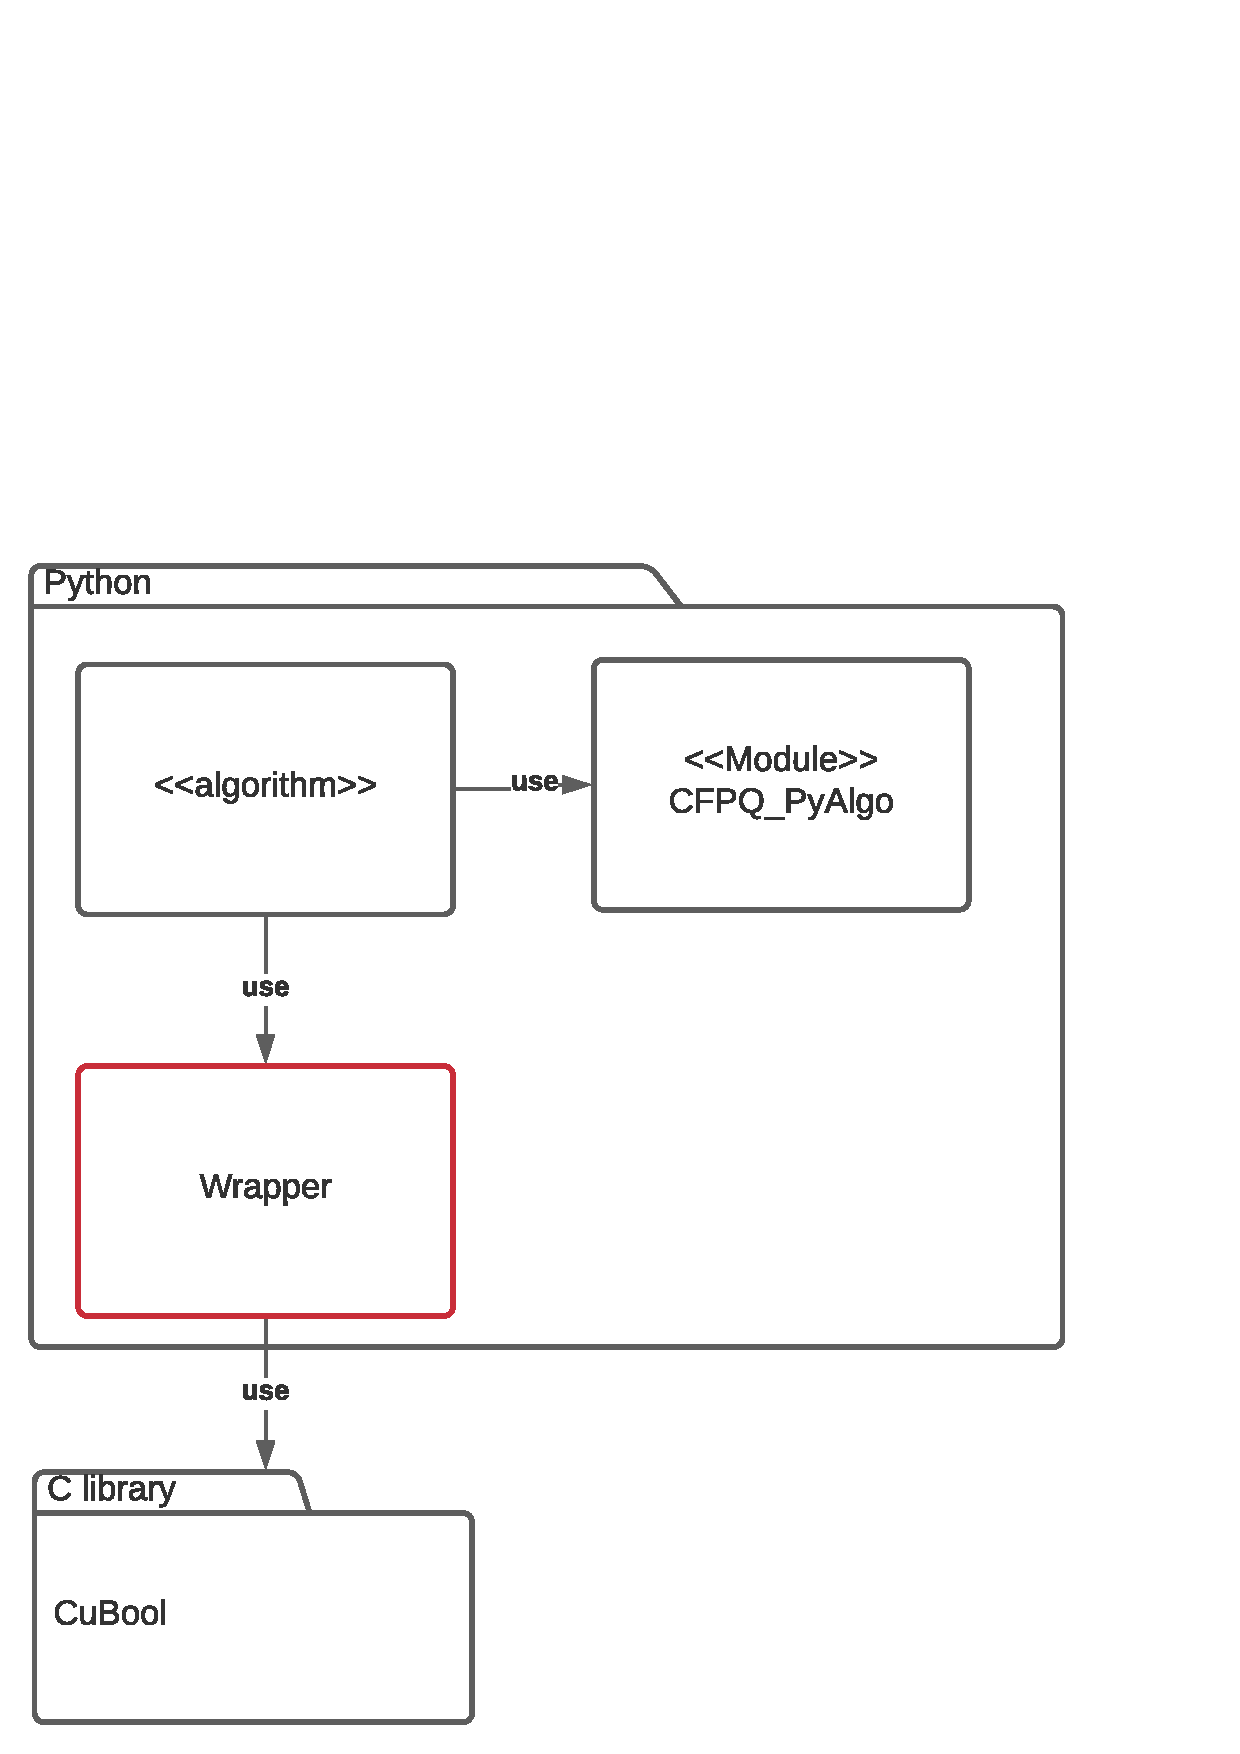
\includegraphics[width=1\linewidth]{pictures/arch.png}
  \caption{Диаграмма последовательностей запуска экспериментов с помощью разработанного инструмента.}
\end{figure}\label{arch}

Перед запуском экспериментов инструмент генерирует данные для соответствующего сценария исполнения. Для этого вызывается \verb|Chunk| \verb|generator|, который выбирает множество начальных вершин графа, на котором будет запущена каждая из реализаций. После чего генерируется множество запросов по определенным заранее шаблонам. Так, \verb|Query| \verb|generator| поддерживает генерацию запросов нескольких видов: в виде регулярного выражения, в виде правил регулярной грамматики и в виде программы на языке Datalog. Создание запросов происходит с помощью конфигурационных файлов, в которых хранятся имена меток на ребрах графа и количество ребер с соответствующей меткой. Благодаря чему удаётся создать запросы с наиболее популярными метками в графе. Шаблоны, по которым формируются запросы выделены в отдельный файл и могут быть изменены. Также, доступен инструмент для подсчета статистики меток в графе, который позволяет создать конфигурационный файл по каждому графу.

Далее, пользователь инициирует выполнение эксперимента на выбранном множестве сценариев. Для каждого из сценариев запускается реализация алгоритма, решающего задачу поиска путей с регулярными ограничениями. После того, как алгоритм закончил исполнение запроса, он возвращает результат в виде числа найденных вершин. В итоге \verb|Scenario orchestrator| сохраняет показатели времени исполнения вычислений в отдельный файл, а также обрабатывает ошибки, которые могли возникнуть во время работы алгоритма. В результате постановки эксперимента отправляется отчет, содержащий информацию о запущенном сценарии, времени исполнения и результате работы алгоритма.
